\section{Описание использованных инструментов}
\pretolerance10000

При выполнении данной проектной работы использовались следующие инструменты: кроссплатформенная система автоматизации сборки программного обеспечения из исходного кода CMake, стандартная библиотека шаблонов С++ STL, контейнерный гипервизор LXD, система подготовки (верстки) документов \LaTeX, инструмент для создания диаграмм PlantUML.\par 
\vspace{\baselineskip}

\subsection{CMake}  
CMake -- это кроссплатформенная система автоматизации сборки программного обеспечения из исходного кода.\par
CMake является по-настоящему кроссплатформенным генератором проектов, позволяющим создавать единые описания проектов для Linux и других Unix–систем (включая Mac OS X) и Windows. Кроме того, CMake стремится максимально использовать фирменные средства генерации сборочных файлов, обладает интеллектуальной системой поиска инструментов сборки и библиотек на конкретной платформе и автоматического конфигурирования. Благодаря этому, система CMake сама устанавливает многие параметры сборочных файлов, которые в других системах управления сборкой приходится устанавливать вручную [1].\par
 
\vspace{\baselineskip}

\subsection{STL} 
STL (Standard Template Library) -- набор согласованных между собой обобщенных алгоритмов, контейнеров, средств доступа к их содержимому и различных вспомогательных функций в C++.\par
Механизм шаблонов встроен в компилятор C++, чтобы дать возможность программистам делать свой код короче за счет обобщенного программирования. Среди существующих стандартных библиотек, реализующих эти механизмы, STL является самой эффективной библиотекой C++ на сегодняшний день [2].\par

\vspace{\baselineskip}

\subsection{LXD} 
LXD (Linux Container Daemon) -- диспетчер контейнеров нового поколения, обеспечивающий опыт работы, схожий с виртуальными машинами, используя вместо них Linux-контейнеры.\par
LXD базируется на API LXC (Application Programming Interface Linux Containers) и ее привязках для различных языков программирования, но при этом инструменты и шаблоны заменены новыми. К числу преимуществ LXD можно отнести его относительную простоту, безопасность по умолчанию, возможность работы с контейнерными образами при создании контейнера (а не с шаблонами) и оптимизированная поддержка состояний контейнера checkpoint и restore для живой миграции [3].\par

\vspace{\baselineskip}

\subsection{LaTeX}
\LaTeX -- это собирательное название для системы подготовки (верстки) документов. Она включает набор инструментов, которые из текстовых файлов, записанных с использованием специального языка разметки формируют готовые к печати документы (как правило в формате PDF). Собственно, \TeX -- это низкоуровневый язык разметки и программирования который лежит в основе этой системы [4].\par
Особенности \LaTeX:
\begin{itemize}
    \item удобное средство для написания технических отчетов и различной документации;
    \item стиль, шрифты, оформление таблиц, рисунков и т.д. согласованы во всём документе;
    \item большие документы можно разбивать на несколько файлов и работать с ними отдельно, в том числе с использованием систем управления версиями;
    \item легко создаются алфавитные указатели, библиографические списки, сноски, ссылки;
    \item удобно включать такие вставки, как исходный код, математические формулы.
    \end{itemize}
\vspace{\baselineskip}

\subsection{PlantUML}
PlantUML -- это инструмент с открытым исходным кодом, позволяющий пользователям создавать диаграммы UML с обычного текстового языка. Язык PlantUML является примером специфического для приложения языка. Он использует программное обеспечение Graphviz для выкладки своих диаграмм.\par
В сравнении с другими известными инструментами для создания диаграмм такими, как Microsoft Visio, Rational Rose, можно выделить следующие преимущества использования PlantUML:
\begin{itemize}
    \item создание диаграмм в виде текста (пример диаграмммы приведен ниже на рисунке 1, ее графическое отображение на рисунке 12), соответственно в любом текстовом редакторе можно произвести рефакторинг, что очень удобно, также текстовый формат дает возможность легко организовывать групповую работу и осуществлять отслеживание изменений в системе контроля версий;
    \item на создание диаграмм требуется меньше времени, чем при создании в любых визуальных редакторах;
    \item гибкий подход к нотации UML -- поддерживая все основные ее элементы, он дает пользователю множество возможностей для их свободного использования в диаграмме, например, очень удобной является поддержка использования вики-разметки в содержимом элементов;
    \item не позволяет создавать больших диаграмм, но это не совсем ограничение -- он распределяет элементы самостоятельно и, естественно, при большом количестве элементов результат начинает быть сомнительным, и лучше диаграмму разделить или уменьшить количество несущественных деталей;
    \item диаграммы PlantUML можно генерировать автоматически [5].
\end{itemize}
\vspace{\baselineskip}
\begin{center}
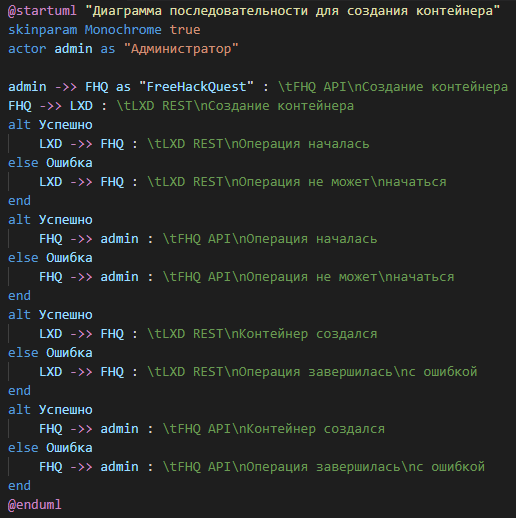
\includegraphics[width=0.65\textwidth]{0}\\
Рисунок 1 -- Текст диаграммы\\
\end{center}
\vspace{\baselineskip}

\subsection{GNU Debugger}
GNU Debugger (GDB) -- переносимый отладчик проекта GNU, способный работать на многих UNIX-подобных системах и производить отладку программ, написанных на различных распространенных компилируемых языках программирования, включая языки Си и C++. GDB является свободным программным обеспечением, распространяемым по лицензии GPL (GNU General Public License) [6].\par
Данный отладчик предлагает широкий список функций, позволяющих контролировать ход выполнения программы:
\begin{itemize}
\item пошаговая отладка с возможностью задать точку остановки программы в требуемом месте или по достижению определенного условия;
\item исследование и изменение значений внутренних переменных программы;
\item вызов внутренних функций программы независимо от ее обычного поведения;
\item предоставление информации о том, что произошло в момент, когда программа остановилась.
\end{itemize}
\clearpage
